\documentclass[]{book}
\usepackage{lmodern}
\usepackage{amssymb,amsmath}
\usepackage{ifxetex,ifluatex}
\usepackage{fixltx2e} % provides \textsubscript
\ifnum 0\ifxetex 1\fi\ifluatex 1\fi=0 % if pdftex
  \usepackage[T1]{fontenc}
  \usepackage[utf8]{inputenc}
\else % if luatex or xelatex
  \ifxetex
    \usepackage{mathspec}
  \else
    \usepackage{fontspec}
  \fi
  \defaultfontfeatures{Ligatures=TeX,Scale=MatchLowercase}
\fi
% use upquote if available, for straight quotes in verbatim environments
\IfFileExists{upquote.sty}{\usepackage{upquote}}{}
% use microtype if available
\IfFileExists{microtype.sty}{%
\usepackage{microtype}
\UseMicrotypeSet[protrusion]{basicmath} % disable protrusion for tt fonts
}{}
\usepackage[margin=1in]{geometry}
\usepackage{hyperref}
\hypersetup{unicode=true,
            pdftitle={A Course in the EMU-SDMS},
            pdfborder={0 0 0},
            breaklinks=true}
\urlstyle{same}  % don't use monospace font for urls
\usepackage{natbib}
\bibliographystyle{apalike}
\usepackage{color}
\usepackage{fancyvrb}
\newcommand{\VerbBar}{|}
\newcommand{\VERB}{\Verb[commandchars=\\\{\}]}
\DefineVerbatimEnvironment{Highlighting}{Verbatim}{commandchars=\\\{\}}
% Add ',fontsize=\small' for more characters per line
\usepackage{framed}
\definecolor{shadecolor}{RGB}{248,248,248}
\newenvironment{Shaded}{\begin{snugshade}}{\end{snugshade}}
\newcommand{\KeywordTok}[1]{\textcolor[rgb]{0.13,0.29,0.53}{\textbf{{#1}}}}
\newcommand{\DataTypeTok}[1]{\textcolor[rgb]{0.13,0.29,0.53}{{#1}}}
\newcommand{\DecValTok}[1]{\textcolor[rgb]{0.00,0.00,0.81}{{#1}}}
\newcommand{\BaseNTok}[1]{\textcolor[rgb]{0.00,0.00,0.81}{{#1}}}
\newcommand{\FloatTok}[1]{\textcolor[rgb]{0.00,0.00,0.81}{{#1}}}
\newcommand{\ConstantTok}[1]{\textcolor[rgb]{0.00,0.00,0.00}{{#1}}}
\newcommand{\CharTok}[1]{\textcolor[rgb]{0.31,0.60,0.02}{{#1}}}
\newcommand{\SpecialCharTok}[1]{\textcolor[rgb]{0.00,0.00,0.00}{{#1}}}
\newcommand{\StringTok}[1]{\textcolor[rgb]{0.31,0.60,0.02}{{#1}}}
\newcommand{\VerbatimStringTok}[1]{\textcolor[rgb]{0.31,0.60,0.02}{{#1}}}
\newcommand{\SpecialStringTok}[1]{\textcolor[rgb]{0.31,0.60,0.02}{{#1}}}
\newcommand{\ImportTok}[1]{{#1}}
\newcommand{\CommentTok}[1]{\textcolor[rgb]{0.56,0.35,0.01}{\textit{{#1}}}}
\newcommand{\DocumentationTok}[1]{\textcolor[rgb]{0.56,0.35,0.01}{\textbf{\textit{{#1}}}}}
\newcommand{\AnnotationTok}[1]{\textcolor[rgb]{0.56,0.35,0.01}{\textbf{\textit{{#1}}}}}
\newcommand{\CommentVarTok}[1]{\textcolor[rgb]{0.56,0.35,0.01}{\textbf{\textit{{#1}}}}}
\newcommand{\OtherTok}[1]{\textcolor[rgb]{0.56,0.35,0.01}{{#1}}}
\newcommand{\FunctionTok}[1]{\textcolor[rgb]{0.00,0.00,0.00}{{#1}}}
\newcommand{\VariableTok}[1]{\textcolor[rgb]{0.00,0.00,0.00}{{#1}}}
\newcommand{\ControlFlowTok}[1]{\textcolor[rgb]{0.13,0.29,0.53}{\textbf{{#1}}}}
\newcommand{\OperatorTok}[1]{\textcolor[rgb]{0.81,0.36,0.00}{\textbf{{#1}}}}
\newcommand{\BuiltInTok}[1]{{#1}}
\newcommand{\ExtensionTok}[1]{{#1}}
\newcommand{\PreprocessorTok}[1]{\textcolor[rgb]{0.56,0.35,0.01}{\textit{{#1}}}}
\newcommand{\AttributeTok}[1]{\textcolor[rgb]{0.77,0.63,0.00}{{#1}}}
\newcommand{\RegionMarkerTok}[1]{{#1}}
\newcommand{\InformationTok}[1]{\textcolor[rgb]{0.56,0.35,0.01}{\textbf{\textit{{#1}}}}}
\newcommand{\WarningTok}[1]{\textcolor[rgb]{0.56,0.35,0.01}{\textbf{\textit{{#1}}}}}
\newcommand{\AlertTok}[1]{\textcolor[rgb]{0.94,0.16,0.16}{{#1}}}
\newcommand{\ErrorTok}[1]{\textcolor[rgb]{0.64,0.00,0.00}{\textbf{{#1}}}}
\newcommand{\NormalTok}[1]{{#1}}
\usepackage{longtable,booktabs}
\usepackage{graphicx,grffile}
\makeatletter
\def\maxwidth{\ifdim\Gin@nat@width>\linewidth\linewidth\else\Gin@nat@width\fi}
\def\maxheight{\ifdim\Gin@nat@height>\textheight\textheight\else\Gin@nat@height\fi}
\makeatother
% Scale images if necessary, so that they will not overflow the page
% margins by default, and it is still possible to overwrite the defaults
% using explicit options in \includegraphics[width, height, ...]{}
\setkeys{Gin}{width=\maxwidth,height=\maxheight,keepaspectratio}
\IfFileExists{parskip.sty}{%
\usepackage{parskip}
}{% else
\setlength{\parindent}{0pt}
\setlength{\parskip}{6pt plus 2pt minus 1pt}
}
\setlength{\emergencystretch}{3em}  % prevent overfull lines
\providecommand{\tightlist}{%
  \setlength{\itemsep}{0pt}\setlength{\parskip}{0pt}}
\setcounter{secnumdepth}{5}
% Redefines (sub)paragraphs to behave more like sections
\ifx\paragraph\undefined\else
\let\oldparagraph\paragraph
\renewcommand{\paragraph}[1]{\oldparagraph{#1}\mbox{}}
\fi
\ifx\subparagraph\undefined\else
\let\oldsubparagraph\subparagraph
\renewcommand{\subparagraph}[1]{\oldsubparagraph{#1}\mbox{}}
\fi

%%% Use protect on footnotes to avoid problems with footnotes in titles
\let\rmarkdownfootnote\footnote%
\def\footnote{\protect\rmarkdownfootnote}

%%% Change title format to be more compact
\usepackage{titling}

% Create subtitle command for use in maketitle
\newcommand{\subtitle}[1]{
  \posttitle{
    \begin{center}\large#1\end{center}
    }
}

\setlength{\droptitle}{-2em}
  \title{A Course in the EMU-SDMS}
  \pretitle{\vspace{\droptitle}\centering\huge}
  \posttitle{\par}
  \author{}
  \preauthor{}\postauthor{}
  \predate{\centering\large\emph}
  \postdate{\par}
  \date{2017-10-08}

\usepackage{booktabs}
\usepackage{amsthm}
\makeatletter
\def\thm@space@setup{%
  \thm@preskip=8pt plus 2pt minus 4pt
  \thm@postskip=\thm@preskip
}
\makeatother

\usepackage{amsthm}
\newtheorem{theorem}{Theorem}[chapter]
\newtheorem{lemma}{Lemma}[chapter]
\theoremstyle{definition}
\newtheorem{definition}{Definition}[chapter]
\newtheorem{corollary}{Corollary}[chapter]
\newtheorem{proposition}{Proposition}[chapter]
\theoremstyle{definition}
\newtheorem{example}{Example}[chapter]
\theoremstyle{definition}
\newtheorem{exercise}{Exercise}[chapter]
\theoremstyle{remark}
\newtheorem*{remark}{Remark}
\newtheorem*{solution}{Solution}
\begin{document}
\maketitle

{
\setcounter{tocdepth}{1}
\tableofcontents
}
\chapter{Prerequisites}\label{prerequisites}

(copy and pasted from EMU manual) A prerequisite that is presumed
throughout this document is the reader's familiarity with basic
terminology in the speech sciences (e.g., familiarity with the
international phonetic alphabet and how speech is annotated at a coarse
and fine grained level). Further, we assume the reader has a grasp of
the basic concepts of the R language and environment for statistical
computing and graphics. For readers new to R, there are multiple, freely
available R tutorials online (e.g.,
\href{https://en.wikibooks.org/wiki/Statistical_Analysis:_an_Introduction_using_R/R_basics}{Statistical
Analysis: an Introduction using R/R\_basics}. R also has a set of very
detailed manuals and tutorials that come preinstalled with R. To be able
to access R's own ``An Introduction to R'' introduction, simply type
\texttt{help.start()} into the R console and click on the link to the
tutorial.

\section{Installing the EMU-SDMS}\label{installing-the-emu-sdms}

(copy and pasted from EMU manual)

1.) R

\begin{itemize}
\tightlist
\item
  Download the R programming language from
  \href{www.cran.r-project.org}{http://www.cran.r-project.org}
\item
  Install the R programming language by executing the downloaded file
  and following the on-screen instructions.
\end{itemize}

2.) emuR

\begin{itemize}
\tightlist
\item
  Start up R.
\item
  Enter \texttt{install.packages("emuR")} after the
  \texttt{\textgreater{}} prompt to install the package. (You will only
  need to repeat this if package updates become available.)
\item
  As the \texttt{wrassp} package is a dependency of the \texttt{emuR}
  package, it does not have to be installed separately.
\end{itemize}

3.) EMU-webApp (prerequisite)

\begin{itemize}
\tightlist
\item
  The only thing needed to use the EMU-webApp is a current HTML5
  compatible browser (Chrome/Firefox/Safari/Opera/\ldots{}). However, as
  most of the development and testing is done using Chrome we recommend
  using it, as it is by far the best tested browser.
\end{itemize}

\section{Installing additional R-packages that are used throughout this
course}\label{installing-additional-r-packages-that-are-used-throughout-this-course}

\begin{itemize}
\tightlist
\item
  ggplot2 for visualization purposes: \texttt{install.packages("emuR")}
\item
  dplyr for data manipulation: \texttt{install.packages("dplyr")}
\end{itemize}

\chapter{Introduction}\label{intro}

You can label chapter and section titles using \texttt{\{\#label\}}
after them, e.g., we can reference Chapter \ref{intro}. If you do not
manually label them, there will be automatic labels anyway, e.g.,
Chapter \ref{methods}.

Figures and tables with captions will be placed in \texttt{figure} and
\texttt{table} environments, respectively.

\begin{Shaded}
\begin{Highlighting}[]
\KeywordTok{par}\NormalTok{(}\DataTypeTok{mar =} \KeywordTok{c}\NormalTok{(}\DecValTok{4}\NormalTok{, }\DecValTok{4}\NormalTok{, .}\DecValTok{1}\NormalTok{, .}\DecValTok{1}\NormalTok{))}
\KeywordTok{plot}\NormalTok{(pressure, }\DataTypeTok{type =} \StringTok{'b'}\NormalTok{, }\DataTypeTok{pch =} \DecValTok{19}\NormalTok{)}
\end{Highlighting}
\end{Shaded}

\begin{figure}

{\centering 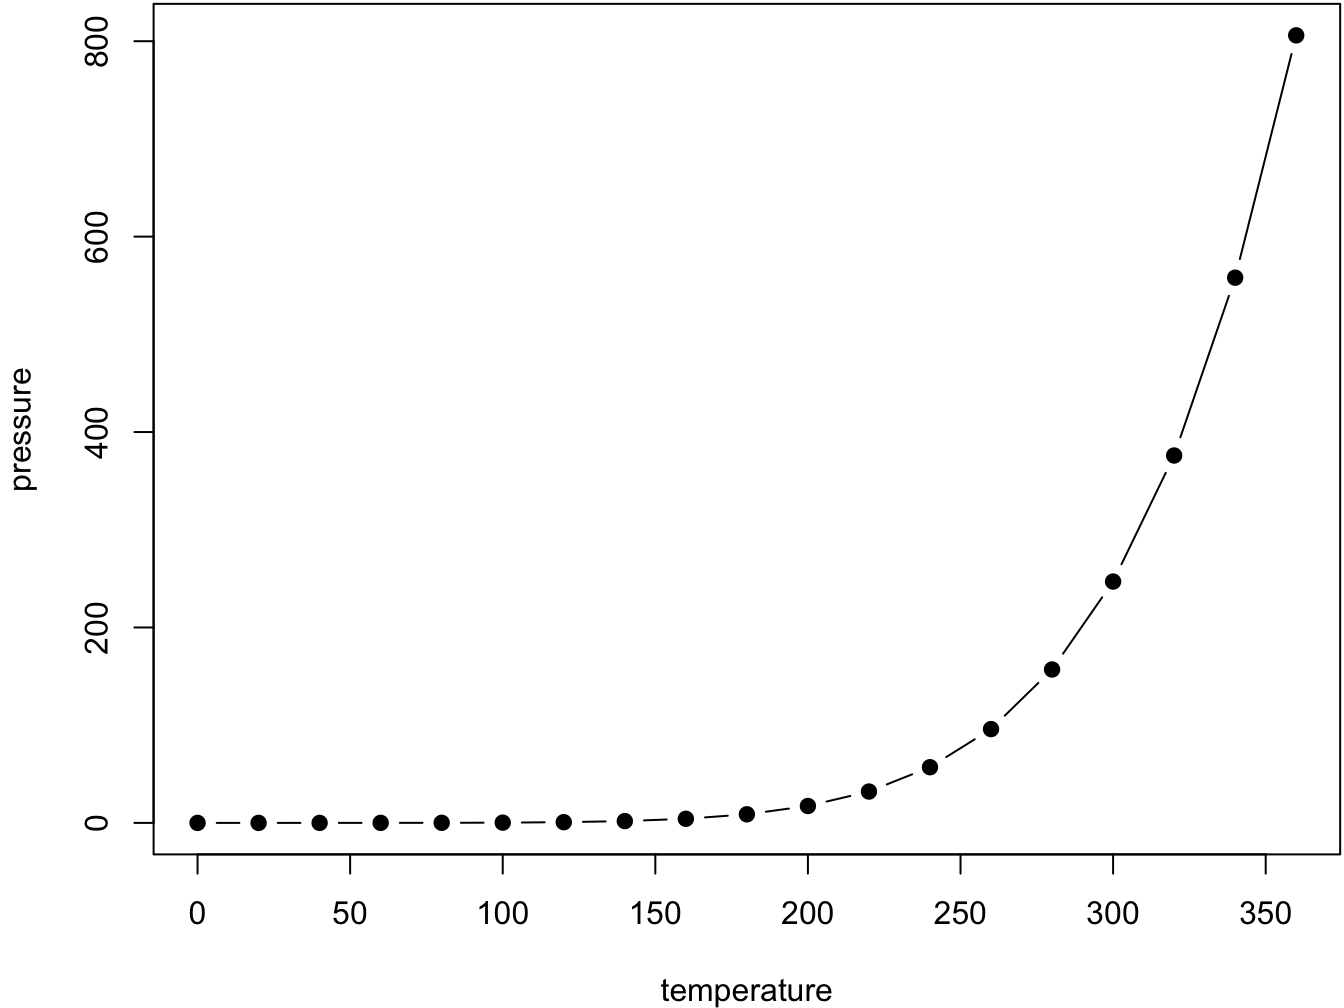
\includegraphics[width=0.8\linewidth]{bookdown-demo_files/figure-latex/nice-fig-1} 

}

\caption{Here is a nice figure!}\label{fig:nice-fig}
\end{figure}

Reference a figure by its code chunk label with the \texttt{fig:}
prefix, e.g., see Figure \ref{fig:nice-fig}. Similarly, you can
reference tables generated from \texttt{knitr::kable()}, e.g., see Table
\ref{tab:nice-tab}.

\begin{Shaded}
\begin{Highlighting}[]
\NormalTok{knitr::}\KeywordTok{kable}\NormalTok{(}
  \KeywordTok{head}\NormalTok{(iris, }\DecValTok{20}\NormalTok{), }\DataTypeTok{caption =} \StringTok{'Here is a nice table!'}\NormalTok{,}
  \DataTypeTok{booktabs =} \OtherTok{TRUE}
\NormalTok{)}
\end{Highlighting}
\end{Shaded}

\begin{table}

\caption{\label{tab:nice-tab}Here is a nice table!}
\centering
\begin{tabular}[t]{rrrrl}
\toprule
Sepal.Length & Sepal.Width & Petal.Length & Petal.Width & Species\\
\midrule
5.1 & 3.5 & 1.4 & 0.2 & setosa\\
4.9 & 3.0 & 1.4 & 0.2 & setosa\\
4.7 & 3.2 & 1.3 & 0.2 & setosa\\
4.6 & 3.1 & 1.5 & 0.2 & setosa\\
5.0 & 3.6 & 1.4 & 0.2 & setosa\\
\addlinespace
5.4 & 3.9 & 1.7 & 0.4 & setosa\\
4.6 & 3.4 & 1.4 & 0.3 & setosa\\
5.0 & 3.4 & 1.5 & 0.2 & setosa\\
4.4 & 2.9 & 1.4 & 0.2 & setosa\\
4.9 & 3.1 & 1.5 & 0.1 & setosa\\
\addlinespace
5.4 & 3.7 & 1.5 & 0.2 & setosa\\
4.8 & 3.4 & 1.6 & 0.2 & setosa\\
4.8 & 3.0 & 1.4 & 0.1 & setosa\\
4.3 & 3.0 & 1.1 & 0.1 & setosa\\
5.8 & 4.0 & 1.2 & 0.2 & setosa\\
\addlinespace
5.7 & 4.4 & 1.5 & 0.4 & setosa\\
5.4 & 3.9 & 1.3 & 0.4 & setosa\\
5.1 & 3.5 & 1.4 & 0.3 & setosa\\
5.7 & 3.8 & 1.7 & 0.3 & setosa\\
5.1 & 3.8 & 1.5 & 0.3 & setosa\\
\bottomrule
\end{tabular}
\end{table}

You can write citations, too. For example, we are using the
\textbf{bookdown} package \citep{R-bookdown} in this sample book, which
was built on top of R Markdown and \textbf{knitr} \citep{xie2015}.

\chapter{An overview of the EMU-SDMS}\label{an-overview-of-the-emu-sdms}

Here is a review of existing methods.

\chapter{Toolchain SpeechRecorder --- MAUS ---
EMU-SDMS}\label{toolchain-speechrecorder-maus-emu-sdms}

Most phonetic research projects involve this workflow:

\begin{enumerate}
\def\labelenumi{\arabic{enumi}.}
\tightlist
\item
  Record speech
\item
  Annotate speech using automatic tools
\item
  Check and correct the generated annotations by hand
\item
  Analyze speech (connecting the primary data with annotations and
  derived signals)
\end{enumerate}

The EMU Speech Database Management System is focused on steps 3 and 4 of
this workflow. For the first two steps, it can very usefully be
complemented by two other tools:
\href{http://www.speechrecorder.org/}{SpeechRecorder} and MAUS (or, more
broadly speaking --- and more correctly, for that matter --- the
\href{https://clarin.phonetik.uni-muenchen.de/BASWebServices}{BAS Web
Services}). This chapter introduces how the tools can be combined --- in
a systematic way, with as little fuss as possible.

\section{What do SpeechRecorder and MAUS
do?}\label{what-do-speechrecorder-and-maus-do}

``SpeechRecorder is a platform independent audio recording software
customized to the requirements of speech recordings''
(\url{http://www.speechrecorder.org/}). To this end, SpeechRecorder lets
you define prompts that participants will read (or otherwise react to)
while you are recording them. At the end of a session, instead of one
large recording of the whole session, you have a set of smaller audio
recordings, each one representing a single prompt.

MAUS (Munich AUtomatic Segmentation) processes audio recordings with
corresponding orthographic transcriptions, and outputs (1) a
corresponding phonetic transcription and (2) a segmentation of the
signal into individual speech sounds. As such, MAUS is a part of the
\href{https://clarin.phonetik.uni-muenchen.de/BASWebServices}{BAS Web
Services}. \footnote{Strictly speaking, MAUS is used in conjunction with
  G2P and possibly Chunker to achieve this result. The whole package is
  often referred to as MAUS, however.}

\section{Different types of prompts}\label{different-types-of-prompts}

Prompts are very often sentences that participants read out aloud
(producing \emph{read speech}). However, this need not be the case.
Prompts may as well be, for example, images that participants have to
name or describe, or written questions that participants answer.

In terms of processing, \emph{read speech} has the advantage that the
researcher already has orthographic transcriptions of all recordings,
because the prompts \emph{are} the transcriptions (this neglects
hesitations, misread utterances, etc.).

For all cases besides read speech, transcriptions have to be prepared.
For read speech, when hesitations etc. need to be considered, the
existing transcriptions need to be corrected (per token). For the time
being, this is out of the scope of this book.\footnote{It will be
  covered, at a later time, in this or a separate chapter.}

\section{Combining the tools}\label{combining-the-tools}

The order of the processing steps is unchangeable: The files have to be
recorded first, then annotated and then analyzed.

However, there are different ways of passing data around between the
tools. For example SpeechRecorder might \emph{export} files into emuDB
format or the EMU-SDMS might \emph{import} files stored in
SpeechRecorder's format. After all, they are separate tools and can be
used individually (although the combination makes great sense).

Moreover, sometimes a database grows, and some new files are recorded
while others have already been annotated or analyzed (which challenges
the ``unchangeable order of processing steps'').

We can see now that we have to convert our data between different
formats. We want to benefit from all tools but keep the conversion work
down to a minimum. In this section, we explain the (currently) best way
to do this. We will import SpeechRecorder's recordings and prompts into
the EMU-SDMS and then use emuR to send the data to MAUS and other BAS
Web Services.

\subsection{Importing recordings and transcriptions into
Emu}\label{importing-recordings-and-transcriptions-into-emu}

\subsubsection{Using the import\_speechRecorder()
function}\label{using-the-import_speechrecorder-function}

The \texttt{import\_speechRecorder()} function is in the making, but
unfortunately not finished yet. We therefore have to resort to the
second-best way of importing SpeechRecorder's results into Emu:

\subsubsection{Using intermediary text
files}\label{using-intermediary-text-files}

SpeechRecorder, per default, saves one .wav file for each prompt. With
additional settings, it will save a .txt file containing the
corresponding prompt along with each .wav file. This is great because it
is exactly what MAUS needs as its input.

The following options must be configured \emph{before recordings are
made}. Note that parts of SpeechRecorder's user interface are in German:

\begin{itemize}
\tightlist
\item
  Under ``Projekt / Einstellungen\ldots{} / Annotation'':

  \begin{itemize}
  \tightlist
  \item
    Under ``Persist'', tick the checkbox that says ``Simple text loader
    writer for annotation template for MAUS processing''
  \item
    Under ``Auto annotation'', tick the checkbox that says ``Prompt
    template auto annotator'' (note that the two checkboxes are very
    similar. Make sure to tick the right one.)
  \end{itemize}
\item
  In your script:

  \begin{itemize}
  \tightlist
  \item
    If you edit the XML file directly: Make sure each of your
    \texttt{\textless{}mediaitem\textgreater{}} elements has the
    attribute \texttt{annotationTemplate="true"}
  \item
    If you use the integrated script editor: Make sure to tick the
    checkbox ``Use as annotation template'' for \emph{every recording}.
  \end{itemize}
\end{itemize}

Now, after your recording session, you will have audio and text files.
In emuR, this combination is called a \emph{txt collection}. We will
thus use the function \texttt{convert\_txtCollection}, to import
SpeechRecorder's files into Emu's format. In the following example, we
will use the sample txt collection included with the emuR package.

\begin{Shaded}
\begin{Highlighting}[]
\CommentTok{# Load the emuR package}
\KeywordTok{library}\NormalTok{(emuR)}

\CommentTok{# Create demo data in directory provided by tempdir()}
\KeywordTok{create_emuRdemoData}\NormalTok{(}\DataTypeTok{dir =} \KeywordTok{tempdir}\NormalTok{())}

\CommentTok{# Import the sample txt collection.}
\CommentTok{# When used with real data, sourceDir should point to the RECS directory of your}
\CommentTok{# SpeechRecorder project.}
\KeywordTok{convert_txtCollection}\NormalTok{(}\DataTypeTok{dbName =} \StringTok{"myEmuDatabase"}\NormalTok{,}
                      \DataTypeTok{sourceDir =} \KeywordTok{file.path}\NormalTok{(}\KeywordTok{tempdir}\NormalTok{(), }\StringTok{"emuR_demoData"}\NormalTok{, }\StringTok{"txt_collection"}\NormalTok{),}
                      \DataTypeTok{targetDir =} \KeywordTok{tempdir}\NormalTok{())}

\NormalTok{dbHandle =}\StringTok{ }\KeywordTok{load_emuDB}\NormalTok{(}\KeywordTok{file.path}\NormalTok{(}\KeywordTok{tempdir}\NormalTok{(), }\StringTok{"myEmuDatabase_emuDB"}\NormalTok{))}
\end{Highlighting}
\end{Shaded}

Now, you have an Emu database. You can inspect it using

\begin{Shaded}
\begin{Highlighting}[]
\KeywordTok{summary}\NormalTok{(dbHandle)}
\end{Highlighting}
\end{Shaded}

or

\begin{Shaded}
\begin{Highlighting}[]
\KeywordTok{serve}\NormalTok{(dbHandle)}
\end{Highlighting}
\end{Shaded}

The database contains all our recordings, and exactly one type of
annotation: orthographic transcription. No phonetic transcription, no
segmentation. The next section will cover that.

\subsection{Feeding the data into
MAUS}\label{feeding-the-data-into-maus}

The .wav and .txt files could have been uploaded on the
\href{https://clarin.phonetik.uni-muenchen.de/BASWebServices/\#!/services/Pipeline}{BAS
web site}, but we will do it using emuR. This is generally less
error-prone and requires less manual work. Moreover, since it is a
scripted way of doing things, we can reproduce it reliably.

To process the data, we make use of several of emuR's functions called
\texttt{runBASwebservice\_...}. They will upload the data to WebMAUS and
accompanying services and save the results directly inside your existing
emuDB (this of course takes some time, depending on the size of your
database and the speed of your internet connection).

\begin{Shaded}
\begin{Highlighting}[]
\KeywordTok{runBASwebservice_g2pForTokenization}\NormalTok{(}\DataTypeTok{handle =} \NormalTok{dbHandle,}
                                    \DataTypeTok{language =} \StringTok{"eng-US"}\NormalTok{,}
                                    \DataTypeTok{transcriptionAttributeDefinitionName =} \StringTok{"transcription"}\NormalTok{,}
                                    \DataTypeTok{orthoAttributeDefinitionName =} \StringTok{"Word"}\NormalTok{)}

\KeywordTok{runBASwebservice_g2pForPronunciation}\NormalTok{(}\DataTypeTok{handle =} \NormalTok{dbHandle,}
                                     \DataTypeTok{language =} \StringTok{"eng-US"}\NormalTok{,}
                                     \DataTypeTok{orthoAttributeDefinitionName =} \StringTok{"Word"}\NormalTok{,}
                                     \DataTypeTok{canoAttributeDefinitionName =} \StringTok{"Canonical"}\NormalTok{)}

\KeywordTok{runBASwebservice_maus}\NormalTok{(}\DataTypeTok{handle =} \NormalTok{dbHandle,}
                      \DataTypeTok{language =} \StringTok{"eng-US"}\NormalTok{,}
                      \DataTypeTok{canoAttributeDefinitionName =} \StringTok{"Canonical"}\NormalTok{,}
                      \DataTypeTok{mausAttributeDefinitionName =} \StringTok{"Phonetic"}\NormalTok{)}
\end{Highlighting}
\end{Shaded}

When the services are finished, we can use

\begin{Shaded}
\begin{Highlighting}[]
\KeywordTok{serve}\NormalTok{(db)}
\end{Highlighting}
\end{Shaded}

to inspect the database with the new annotations. This time, it includes
segmentation into words and phonemes, canonical phonetic transcription
and realized phonetic transcription.

This chapter described the current best practice of combining
SpeechRecorder, MAUS and the EMU-SDMS to fit a typical phonetic project
workflow.

\chapter{The EMU-webApp}\label{the-emu-webapp}

Some \emph{significant} applications are demonstrated in this chapter.

\section{Example one}\label{example-one}

\section{Example two}\label{example-two}

\chapter{Creating segment lists and trackdata
objects}\label{creating-segment-lists-and-trackdata-objects}

We have finished a nice book.

\chapter{Wrassp and the application of
DSP}\label{wrassp-and-the-application-of-dsp}

We have finished a nice book.

\chapter{Annotation types and the Emu
Query-language}\label{annotation-types-and-the-emu-query-language}

We have finished a nice book.

\bibliography{packages.bib,book.bib}


\end{document}
